% \iffalse meta-comment ---------------------------------------------
% Copyright (C) Shanghai Jiao Tong University
% The definition in this file is referred to the Visual Identity System
% from Shanghai Jiao Tong University (SJTU). 
% See https://vi.sjtu.edu.cn for more information.
% 
% SJTUG implements the design but doesn't hold the copyright.
% Any commercial usage in this file should be acknowledged by
% the administration of SJTU.
% More information about the license,
% see https://vi.sjtu.edu.cn/index.php/articles/bulletin/16. 
% ------------------------------------------------------------------- \fi
% \iffalse
%<*package>
\NeedsTeXFormat{LaTeX2e}
\ProvidesPackage{sjtucover}[2022/03/21 cover library for sjtubeamer v2.5.7]
%</package>
% \fi
% \CheckSum{0}
% \StopEventually{}
% \iffalse
%<*package>
% ------------------------------------------------------------------- \fi
%
% \subsection{Cover Library}
%   This library provides the template for the title page and the bottom page.
%
%   \subsubsection{Load Packages}
%
%   Load SJTU VI Library to get the definition on shapes. This will also provide \verb"\sjtubeamer@compatible" option.
%    \begin{macrocode}
\RequirePackage{sjtuvi}
%    \end{macrocode}
%
%   \subsubsection{Define Option}
%
%    \begin{macrocode}
\DefineOption{cover}{lang}{cn}
\DefineOption{cover}{lang}{en}
\@ifclassloaded{ctexbeamer}{\ExecuteOptionsBeamer{cn}}{
  \ExecuteOptionsBeamer{en}}
\ProcessOptionsBeamer
%    \end{macrocode}
%
%   \subsubsection{Logo}
%   \paragraph{max.}
%    \begin{macrocode}
%<*max>
\defbeamertemplate*{logo}{max}{\resizebox{!}{1cm}{\sjtubadge}}
%</max>
%    \end{macrocode}
%
%   \paragraph{default.}
%    \begin{macrocode}
\if\EqualOption{cover}{lang}{cn}
  \defbeamertemplate*{logo}{default}{\resizebox{!}{0.7cm}{\cnlogo}}
\else
  \defbeamertemplate*{logo}{default}{\resizebox{!}{0.7cm}{\enlogo}}
\fi
%    \end{macrocode}
%
%    \subsubsection{Title Graphic}
%    \paragraph{maxplus.}
%    \begin{macrocode}
%<*maxplus>
\defbeamertemplate*{titlegraphic}{maxplus}{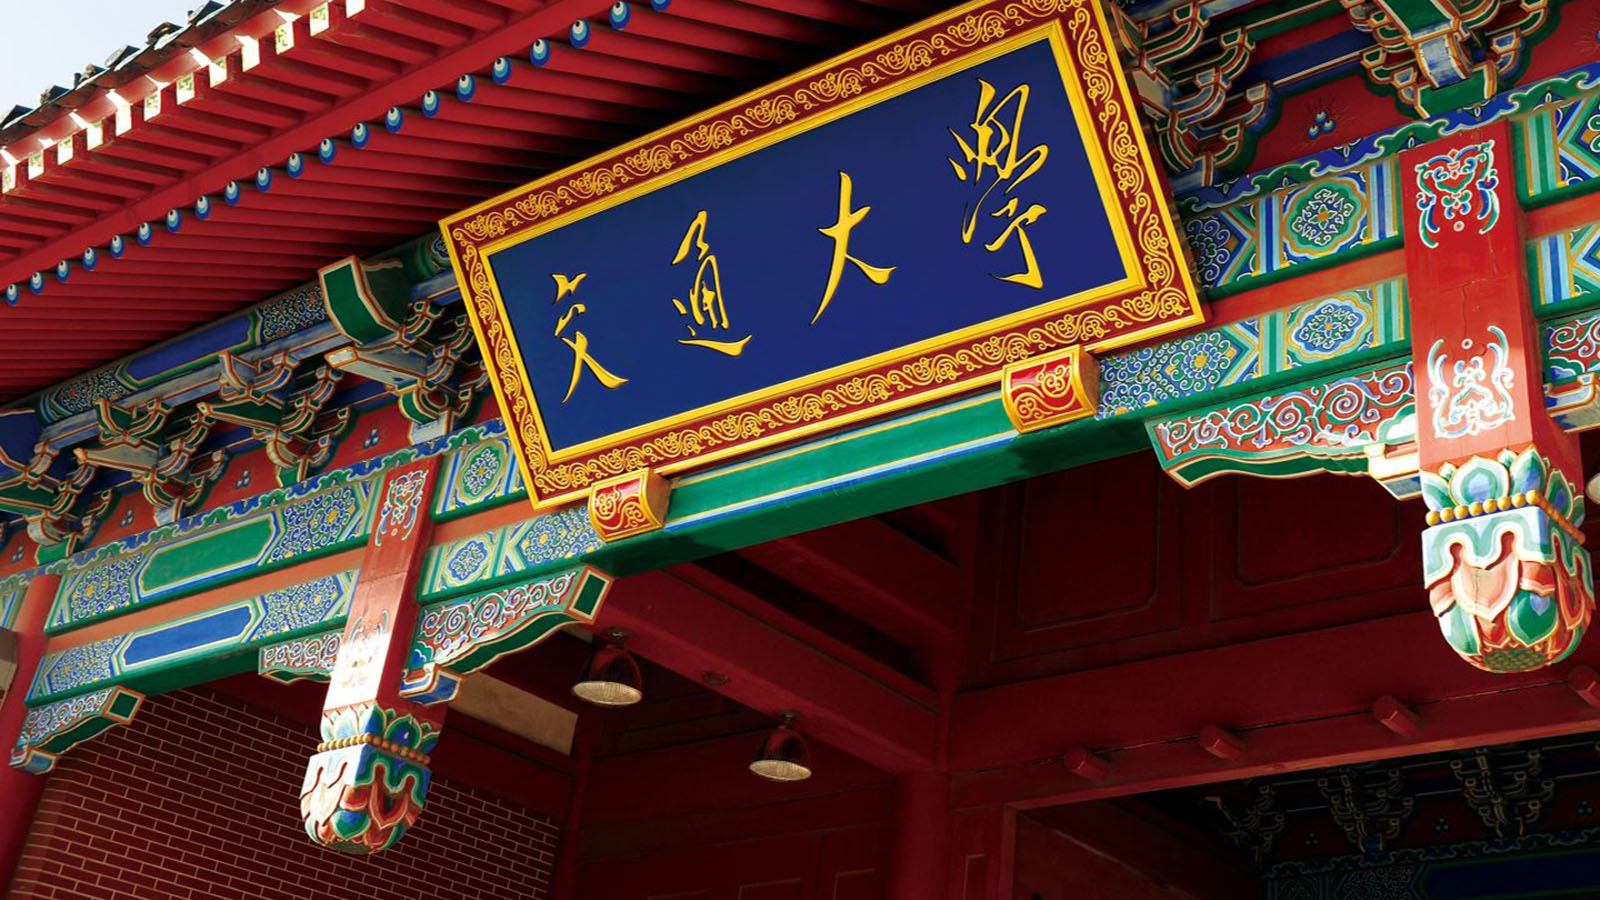
\includegraphics{vi/sjtuphoto.jpg}}
%</maxplus>
%    \end{macrocode}
%
%    \paragraph{max.}
%    \begin{macrocode}
%<*max>
\defbeamertemplate*{titlegraphic}{max}{\sjtubg[opacity=0.2]}
%</max>
%    \end{macrocode}
%
%    \paragraph{min.}
%    \begin{macrocode}
%<*min>
\defbeamertemplate*{titlegraphic}{min}{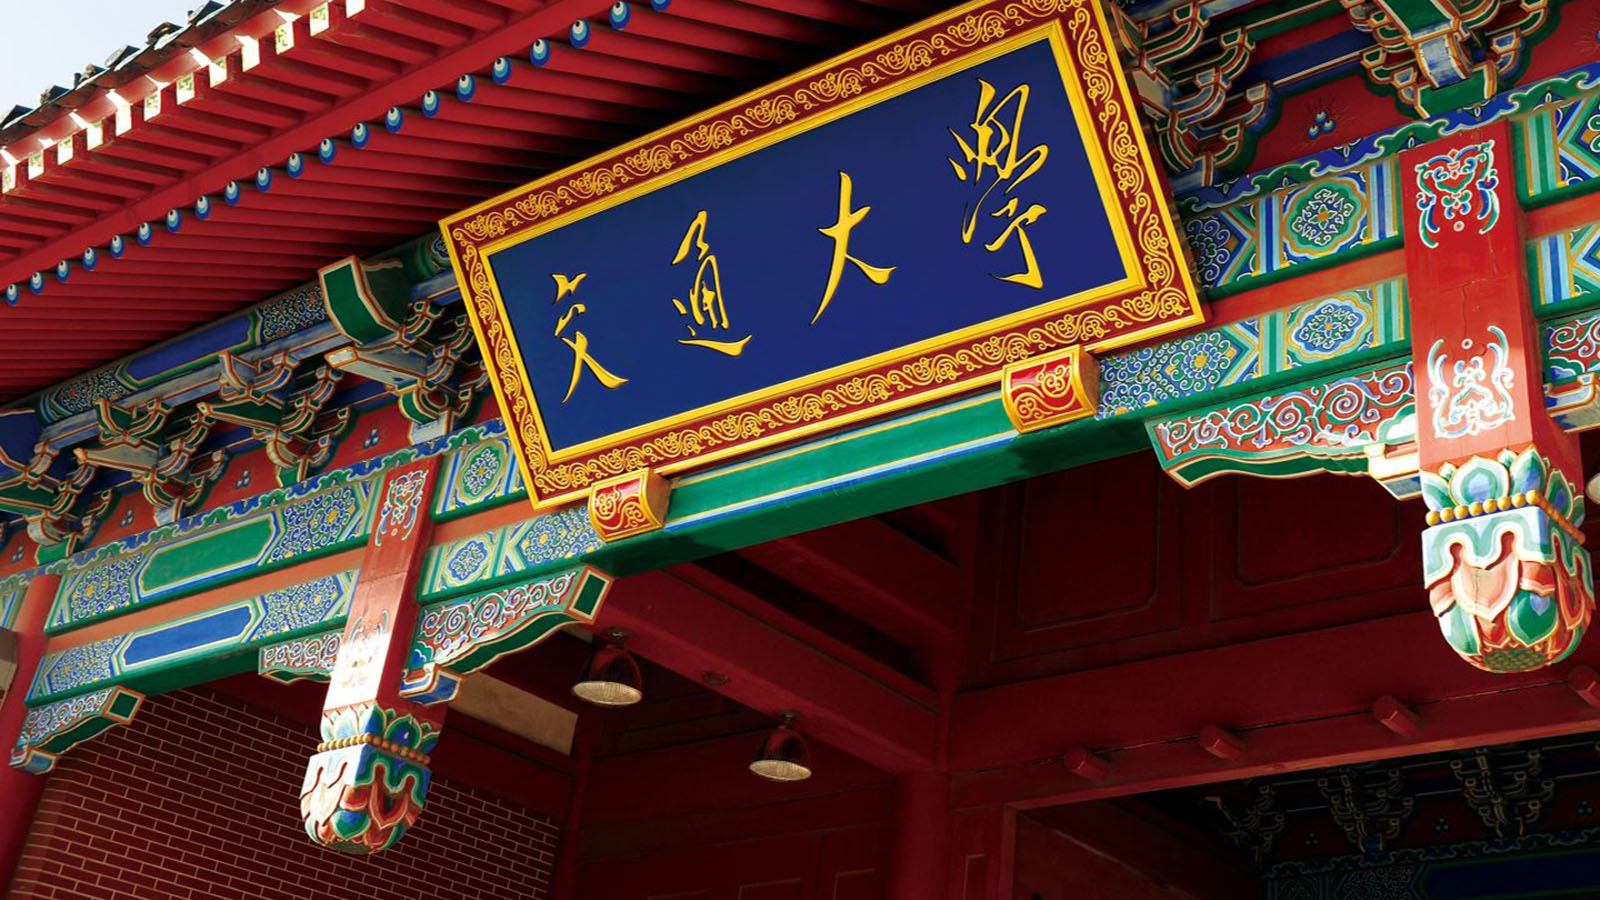
\includegraphics{vi/sjtuphoto.jpg}}
%</min>
%    \end{macrocode}
%
%    \paragraph{my.}
%    \begin{macrocode}
%<*my>
\defbeamertemplate*{titlegraphic}{my}{
  %
  % Developer could define your title graphic here for "my"...
  %
}
%</my>
%    \end{macrocode}
%
%   \subsubsection{Title Page}
%  
%   \paragraph{maxplus.}
%    \begin{macrocode}
%<*maxplus>
\defbeamertemplate*{title page}{maxplus}[1][]
{
  \nointerlineskip%
  \vbox{}
  \vfill
  \begingroup
  \usebeamercolor{palette primary}% 
  \begin{tikzpicture}[overlay,
      xshift=-0.12\paperwidth,
      yshift=-0.53\paperheight]
    \pgfmathsetlengthmacro{\outslant}{1.02\paperwidth}
    \node[inner sep=0, outer sep=0]
      at (0.57\paperwidth,0.5\paperheight){
        \resizebox{!}{1.06\paperheight}{\vphantom{-}\inserttitlegraphic}};
    \fill[color=white] (0,0) rectangle(1.1\paperwidth,3.9);
    \fill[color=bg]  (0,-0.1\paperheight) rectangle(1.1\paperwidth,3.88);
    \node[anchor=north west, text width=.8\paperwidth]
    at (0.11\paperwidth,3.6){%
    \usebeamercolor[fg]{title}
    \ifx\insertsubtitle\@empty%
      {\huge\bfseries\inserttitle}\\
      \else%
      {\Large\bfseries\inserttitle}\\
      {\small\insertsubtitle}\\
    \fi%
    };
    \node[anchor=south west, text width=.8\paperwidth] at (0.11\paperwidth,0.45){%
      {\usebeamercolor[fg]{author}\small\insertauthor\par}
        {\usebeamercolor[fg]{institute}\small\insertinstitute\par}
        {\usebeamercolor[fg]{date}\small\insertdate}%
    };
    \node[anchor=south east, inner sep=0, outer sep=0] at (\outslant,0.5){
      \usebeamercolor[fg]{palatte primary}
      \resizebox{!}{1cm}{\vphantom{-}\usebeamertemplate{logo}}
    };
  \end{tikzpicture}
  \endgroup
  \vfill
}
%</maxplus>
%    \end{macrocode}
%  
%   \paragraph{max.}
%    \begin{macrocode}
%<*max>
\defbeamertemplate*{title page}{max}[1][]
{
  \nointerlineskip
  \vbox{}
  \usebeamercolor{palette primary}
  \begin{tikzpicture}[overlay]
    \fill [palette primary.bg] (-0.2*\the\paperwidth,-1*\the\paperheight)
    rectangle (1*\the\paperwidth, 0.3*\the\paperheight);
    \node [palette primary.fg, inner sep=0pt]
    at (0.45\paperwidth-6pt,-0.4*\the\paperheight)
    {\resizebox{1.3\paperwidth}{!}{\inserttitlegraphic}};
  \end{tikzpicture}
  \vfill
  \begingroup
  \begin{beamercolorbox}[sep=8pt,#1,center]{title}
    \usebeamerfont{title}\inserttitle\par%
    \ifx\insertsubtitle\@empty%
    \else%
      \vskip0.25em%
      {\usebeamerfont{subtitle}\insertsubtitle\par}%
    \fi%     
  \end{beamercolorbox}%
  \vskip1em\par
  \begin{beamercolorbox}[sep=8pt,#1,center]{author}
    \usebeamercolor[fg]{palette primary}
    \usebeamerfont{author}\insertauthor
  \end{beamercolorbox}
  \begin{beamercolorbox}[sep=8pt,#1,center]{institute}
    \usebeamercolor[fg]{palette primary}
    \usebeamerfont{institute}\normalsize\insertinstitute
  \end{beamercolorbox}
  \begin{beamercolorbox}[sep=8pt,#1,center]{date}
    \usebeamercolor[fg]{palette primary}
    \usebeamerfont{date}\insertdate
  \end{beamercolorbox}
  \endgroup
  \vfill
}
%</max>
%    \end{macrocode}
%
%   \paragraph{min.}
%   Declare two fadings: center fade and fade right. The center fade provides a radial fading on the right side of the title page. The fade right provides a linear fading to avoid the collision on the text in the left.
%    \begin{macrocode}
%<*min>
\tikzfading[
  name=center fade,
  inner color=transparent!0,
  outer color=transparent!15
]
\tikzfading[
  name=fade right,
  left color=transparent!0,
  right color=transparent!100
]
%    \end{macrocode}
%
%    \begin{macrocode}
\defbeamertemplate*{title page}{min}[1][]
{
  \vbox{}
%    \end{macrocode}
%   The background of the title page is implemented by a TikZ rectangle, which avoids the changing on \verb"background canvas" beamer color. 
%
%   In this definition environment, you could not change the beamer color. The older version redefines \verb"maketitle" command and switches the \verb"background canvas" color, which is harmful for decoupling. 
%
%   Use TikZ rectangle also avoids the unexpected shift because the risk of redefining the internal command is avoided. If there is any text before the title page, the \verb"\maketitle" will start from a new page.
%    \begin{macrocode}
  \usebeamercolor{palette primary}
  \begin{tikzpicture}[overlay]
    \fill [palette primary.bg] (-0.2*\the\paperwidth,-1*\the\paperheight)
    rectangle (1*\the\paperwidth, 0.2*\the\paperheight);
  \end{tikzpicture}
%    \end{macrocode}
%   WARNING: The pattern in the title page is now deprecated for the unstability of the \verb"fadings" library in TikZ. If you want to use the pattern, please uncomment the code segement manually. The interface of \verb"stamparry" is functional.
%   If it is in draftmode or it is not compatible, no pattern will get rendered.
%   Otherwise, the fade tile of stamp array will get covered on top of the background rectangle.
%   \verb"stamparray" is defined in \verb"SJTUvi". Then, a fade right covers this array layer and a center fade covers the previous result.
%    \begin{macrocode}
  \ifx\sjtubeamer@compatible\sjtubeamer@compatible@false
  \else
    \ifbeamer@draftmode%
    \else%
      \begin{tikzpicture}[overlay]
        \stamparray{20pt}
        {(-0.2*\the\paperwidth,-1*\the\paperheight)}
        {(1*\the\paperwidth, 0.2*\the\paperheight)}
        \fill [bg,path fading=fade right]
        (-0.2*\the\paperwidth,-1*\the\paperheight) rectangle
        (1*\the\paperwidth, 0.2*\the\paperheight);
        \fill [bg,path fading=center fade,xshift=-10pt,yshift=-20pt]
        (0.2*\the\paperwidth,0) circle [radius=\the\paperwidth];
      \end{tikzpicture}
    \fi%
  \fi
%    \end{macrocode}
%   Set a constraint in the vertical mode to make the following contents centered in the middle of the slide.
%    \begin{macrocode}
  \vfill
  \begingroup
  \centering
%    \end{macrocode}
%   \verb"resizebox" is used to adapt to all size of logo into 1cm height one. And it is the same in outer theme to make a 0.7cm logo. 
%   The institute is in \TeX{} code for typesetting. \verb"\beamer@shortinstitute" meta is used to avoid compressing on \verb"\par", while \verb"\insertinstitute" will force the input to spread on one signle line. The mode to use is depended on the \verb"language" option. Super small font could be made by \verb"fontsize".
%   Here, we use the option from inner to get the language setting, if this package is used independently, only chinese mode is available.
%    \begin{macrocode}
  \begin{beamercolorbox}{palette primary}
    \vskip8pt
    \hbox{
      \hskip-4pt{\resizebox{!}{1cm}{\vphantom{-}\usebeamertemplate{logo}}}
      \ifx\insertinstitute\@empty%
      \else
      \ifx\insertlogo\@empty%
        \else
        {\hskip0pt \vrule width0.5pt}\hskip3pt
      \fi
      \if\EqualOption{inner}{lang}{en}
      \vbox to 1cm{
          \vfill
          \vbox{
            \offinterlineskip
            \noindent \strut
            \baselineskip 0pt \lineskip -2pt
            \scriptsize\textsc{\beamer@shortinstitute}
            \strut
          }
          \vfill
        }
      \else
      \vbox{
        \fontsize{13pt}{0pt}\selectfont
        \insertinstitute
        \par\noindent\vskip0.15em
        \fontsize{5pt}{0pt}\selectfont
        \textsc{\insertshortinstitute}
        \baselineskip 3.2pt
        \par~
      }
      \fi
      \fi%
    }
    \vskip8pt
  \end{beamercolorbox}
%    \end{macrocode}
%   Insert title, subtitle, author, and date.
%    \begin{macrocode}
  \begin{beamercolorbox}[sep=8pt,#1]{title}
    \usebeamerfont{title}\inserttitle\par%
    \ifx\insertsubtitle\@empty%
    \else%
      \vskip0.25em%
      {\usebeamerfont{subtitle}\insertsubtitle\par}%
    \fi%     
  \end{beamercolorbox}%
  \vskip1em\par
  \begin{beamercolorbox}[sep=8pt,#1]{author}
    \usebeamerfont{author}\insertauthor
  \end{beamercolorbox}
  \begin{beamercolorbox}[sep=8pt,#1]{date}
    \usebeamerfont{date}\insertdate
  \end{beamercolorbox}
%    \end{macrocode}
%   Here insert the titlegraphic. The node position is set to \verb"above left" to make sure the bottom of the picture is aligned to the bottom of the date line.
%    \begin{macrocode}
  \usebeamercolor{palette primary}% 
  \ifx\inserttitlegraphic\@empty%
  \else
    \begin{tikzpicture}[overlay,yshift=0.77em]
      \node (pic) [fg, above left] at (0.88*\the\paperwidth,0)
      {\resizebox{0.3\paperwidth}{!}{\inserttitlegraphic}};
      \draw[decoration={
            stampline,
            segment length=8pt,
            path has corners=true,
          },decorate,fg]
      (pic.north west) --
      (pic.north east) --
      (pic.south east) --
      (pic.south west) -- cycle;
    \end{tikzpicture}
  \fi
  \endgroup
  \vskip0.5em
  \vfill
}
%</min>
%    \end{macrocode}
%  
%   \paragraph{my.}
%    \begin{macrocode}
%<*my>
\defbeamertemplate*{title page}{my}[1][]{
  %
  % Developer could implement your own title page template here...
  % or use "my" theme first, then implement your title page 
  % in a different style file mycover.sty with:
  %    \defbeamertemplate*{title page}{<another name>}[1][]{<Your implementation>}
  %    \defbeamertemplatealias{title page}{my}{<another name>}
  % and in the main.tex:
  %    \usetheme[my]{sjtubeamer}\usepackage{mycover}
  %
}
%</my>
%    \end{macrocode}
%
% \subsubsection{Bottom Page}
%
%  \begin{macro}{\bottomthanks}
%  The "Thank You" caption in the bottom page. Redefine this command will change the bottom page caption.
%    \begin{macrocode}
\if\EqualOption{cover}{lang}{cn}%
  \newcommand{\bottomthanks}{谢\,谢}
\else%
  \newcommand{\bottomthanks}{Thank You}
\fi%
%    \end{macrocode}
%  \end{macro}
%
%   Bottom page could be generated by \verb"\makebottom" command.
%
%   \paragraph{maxplus.}
%    \begin{macrocode}
%<*maxplus>
\tikzfading[name=fade right img,
  left color=transparent!20,
  right color=transparent!100]
\defbeamertemplate*{bottom page}{maxplus}[1][]
{
  \nointerlineskip
  \vbox{}
  \begin{tikzpicture}[overlay]
    \usebeamercolor{palette primary}
    \fill[palette primary.bg] (-0.2\paperwidth,-\paperheight)
    rectangle (\paperwidth, 0.5\paperheight);
  \end{tikzpicture}
  \vfill
  \begin{beamercolorbox}[sep=0pt]{empty}
    \usebeamercolor{structure}
    \begin{tikzpicture}[overlay,xshift=0.54\paperwidth,yshift=-0.41\paperheight]
      \begin{scope}
        \clip (-0.66\paperwidth,0.06\paperheight)
        rectangle (0.43\paperwidth,0.53\paperheight);
        \node [anchor=north] at (0,0.645\paperheight) {
          \resizebox{1.33\paperwidth}{!}{\inserttitlegraphic}};
        \fill[structure.fg!50!black,path fading=fade right img]
        (-0.66\paperwidth,0.06\paperheight)
        rectangle (0.43\paperwidth,0.53\paperheight);
        \node[white] at (-0.45\paperwidth,0.3\paperheight)
        {\resizebox{!}{0.115\paperheight}{\vphantom{-}\usebeamertemplate{logo}}};
        \node [right, white] at (-0.75\paperwidth, 0.15\paperheight) 
        {\resizebox{1.25\paperwidth}{!}{\sjtugate}};
      \end{scope}
      \node at (-0.13\paperwidth,0.7\paperheight) {
        \usebeamercolor[fg]{title}
        \LARGE \bfseries \bottomthanks
      };
    \end{tikzpicture}
  \end{beamercolorbox}
  \vfill
}
%</maxplus>
%    \end{macrocode}
%
%   \paragraph{max.}
%    \begin{macrocode}
%<*max>
\defbeamertemplate*{bottom page}{max}[1][]
{
  \nointerlineskip
  \vbox{}
  \usebeamercolor{palette primary}
  \usebeamercolor{structure}
  \begin{beamercolorbox}[sep=0pt]{empty}
    \begin{tikzpicture}[overlay,yshift=0.25\paperwidth]
      \def\leftw{0.215\paperwidth}
      \def\midw{0.435\paperwidth}
      \def\rightw{0.655\paperwidth}
      \fill[palette primary.bg] (-0.2\paperwidth,-1.2\paperheight) rectangle
      (\paperwidth, 0.1\paperheight);
      \fill[palette primary.fg] (\leftw,0.1\paperheight)
      -- (\leftw,-0.5\paperheight)
      -- (\midw,-0.65\paperheight)
      -- (\rightw,-0.5\paperheight)
      -- (\rightw,0.1\paperheight) -- cycle;
      \fill[palette primary.fg] (\leftw,-0.53\paperheight)
      -- (\leftw,-0.59\paperheight)
      -- (\midw,-0.74\paperheight)
      -- (\rightw,-0.59\paperheight)
      -- (\rightw,-0.53\paperheight)
      -- (\midw,-0.68\paperheight) -- cycle;
      \node[black] at (\midw,-0.65\paperheight) {
        \resizebox{1.25\paperwidth}{!}{\inserttitlegraphic}};
      \node at (\midw,-0.2\paperheight) {
        \resizebox{3cm}{!}{\hphantom{-}\usebeamertemplate{logo}}};
      \node at (\midw,-0.45\paperheight) {
        \usebeamercolor[bg]{palette primary}
        \LARGE \bfseries\bottomthanks};
    \end{tikzpicture}
  \end{beamercolorbox}
}
%</max>
%    \end{macrocode}
%
%   \paragraph{min.}
%    \begin{macrocode}
%<*min>
\defbeamertemplate*{bottom page}{min}[1][]
{
%    \end{macrocode}
%   Enter vertical mode.
%    \begin{macrocode}
  \vbox{}
%    \end{macrocode}
%   Create the background canvas and the three overlapping circles in the right. Use \verb"scope" to define the influence range. And use \verb"\clip" to make the clipping in the current range.
%    \begin{macrocode}
  \usebeamercolor{palette primary}
  \usebeamercolor{palette secondary}
  \begin{tikzpicture}[overlay,yshift=-80pt]
    \def\w{\the\paperwidth}%
    \def\h{\the\paperheight}%
    \fill [palette primary.bg] (-0.2*\w,-1*\h) rectangle (1*\w, 0.5*\h);
    \begin{scope}[fill=palette primary.bg!50!palette primary.fg,fill opacity=0.15]
      \clip (0.63*\w,1.05*\h) circle (1*\h);
      \fill (0.14*\w,-0.95*\h) circle (1.67*\h);
    \end{scope}
    \begin{scope}
      [fill=palette secondary.bg!50!palette primary.bg!70!palette primary.fg,
        fill opacity=0.15]
      \clip[xshift=26pt] (0.95*\w,-0.67*\h) circle (1.17*\h);
      \fill
      (0.14*\w,-0.95*\h) circle (1.67*\h)
      (0.63*\w,1.05*\h) circle (1*\h);
    \end{scope}
  \end{tikzpicture}
%    \end{macrocode}
%   Insert the logo in the crossing center of the overlapping circles.
%    \begin{macrocode}
  \vfill
  \usebeamercolor[fg]{palette primary}
  \begingroup
  \raggedleft
  \resizebox{!}{1cm}{\vphantom{-}\usebeamertemplate{logo}}
%    \end{macrocode}
%   Inset the ``thank you'' quote and the title of this beamer. Notice that three \verb"\vfill" divide the frame into three portions with final adjust using \verb"\vskip".
%    \begin{macrocode}
  \vfill
  \vskip6em
  \begin{beamercolorbox}[sep=8pt]{title}
    \usebeamerfont{title}\noindent\bottomthanks
    \vskip1em%
    \usebeamerfont{subtitle}
    \insertauthor
    \ifx\insertauthor\@empty
    \else
      \ifx\inserttitle\@empty
      \else~$\cdot$~\fi
    \fi
    \inserttitle
  \end{beamercolorbox}%
  \vfill
  \vskip3.5em
  \endgroup
}
%</min>
%    \end{macrocode}
%
%   \paragraph{my.}
%    \begin{macrocode}
%<*my>
\defbeamertemplate*{bottom page}{my}[1][]
{
  %
  % Developer could implement your own bottom page template here...
  % or use "my" theme first, then implement your title page 
  % in a different style file mycover.sty with:
  %    \defbeamertemplate*{bottom page}{<another name>}[1][]{<Your implementation>}
  %    \defbeamertemplatealias{bottom page}{my}{<another name>}
  % and in the main.tex:
  %    \usetheme[my]{sjtubeamer}\usepackage{mycover}
  %
}
%</my>
%    \end{macrocode}
%
%  \subsubsection{Name Translation}
%     Refer to the default configuration of \verb"ctexbeamer" for the following values. But this doesn't support \verb"\ctexset{}" to modify the headings, since it is not obvious to obtain the ``pure'' number value from the \verb"number" setting. 
%     You could only redefine the internal macro to achieve that.
%
%  \begin{macro}{\sjtubeamer@cover@partnumber}
%    Part number based on different languages and whether the \verb"ctexbeamer" class is loaded.
%    \begin{macrocode}
\if\EqualOption{cover}{lang}{cn}%
  \@ifclassloaded{ctexbeamer}{
%    \end{macrocode}
%    \verb"\chinese" macro is only available in \verb"zhnumber" package, loaded by \verb"ctexbeamer".
%    \begin{macrocode}
    \def\sjtubeamer@cover@partnumber{\chinese{part}}
  }{\def\sjtubeamer@cover@partnumber{\insertromanpartnumber}}
\else%
  \def\sjtubeamer@cover@partnumber{\insertromanpartnumber}
\fi
%    \end{macrocode}
%  \end{macro}
%
%  \begin{macro}{\sjtubeamer@cover@partname}
%    Part name based on different languages and whether the \verb"ctexbeamer" class is loaded.
%    \begin{macrocode}
\if\EqualOption{cover}{lang}{cn}%
  \@ifclassloaded{ctexbeamer}{
    \def\sjtubeamer@cover@partname{第\sjtubeamer@cover@partnumber{}部分}
  }{\def\sjtubeamer@cover@partname{第~\sjtubeamer@cover@partnumber~部分}}
\else%
  \def\sjtubeamer@cover@partname{\partname~\sjtubeamer@cover@partnumber}
\fi%
%    \end{macrocode}
%  \end{macro}
%
%  \begin{macro}{\sjtubeamer@cover@sectionnumber}
%    The section number definition.
%    \begin{macrocode}
\def\sjtubeamer@cover@sectionnumber{\insertsectionnumber}
%    \end{macrocode}
%  \end{macro}
%
%  \begin{macro}{\sjtubeamer@cover@sectionname}
%    Section name based on different languages.
%    \begin{macrocode}
\if\EqualOption{cover}{lang}{cn}%
  \def\sjtubeamer@cover@sectionname{第~\sjtubeamer@cover@sectionnumber~节}
\else
  \def\sjtubeamer@cover@sectionname{\sectionname~\sjtubeamer@cover@sectionnumber}
\fi
%    \end{macrocode}
%  \end{macro}
%
%  \begin{macro}{\sjtubeamer@cover@subsectionnumber}
%    Section number based on different languages.
%    \begin{macrocode}
\if\EqualOption{cover}{lang}{cn}%
  \def\sjtubeamer@cover@subsectionnumber{\arabic{section}.\arabic{subsection}}
\else
  \def\sjtubeamer@cover@subsectionnumber{\insertsubsectionnumber}
\fi
%    \end{macrocode}
%  \end{macro}
%
%  \begin{macro}{\sjtubeamer@cover@subsectionname}
%    Subsection name based on different languages.
%    \begin{macrocode}
\if\EqualOption{cover}{lang}{cn}%
  \def\sjtubeamer@cover@subsectionname{第~\sjtubeamer@cover@subsectionnumber~小节}
\else
  \def\sjtubeamer@cover@subsectionname{\subsectionname~\sjtubeamer@cover@subsectionnumber}
\fi
%    \end{macrocode}
%  \end{macro}
%
%  \subsubsection{Part Page}
%
%  \paragraph{maxplus.}
%    \begin{macrocode}
%<*maxplus>
\defbeamertemplate*{part page}{maxplus}[1][]
{
  \nointerlineskip
  \vbox{}
  \usebeamercolor{palette primary}
  \def\sjtubeamer@logocolor{palette primary.fg}
  \begin{tikzpicture}[overlay]
    \fill [palette primary.bg] (-0.2*\the\paperwidth,-1*\the\paperheight)
    rectangle (1*\the\paperwidth, 0.3*\the\paperheight);
    \node [right, palette primary.fg] at (-0.2*\the\paperwidth, -0.6*\the\paperheight) {\resizebox{1.25\paperwidth}{!}{\sjtugate}};
  \end{tikzpicture}
  \vfil
  \begingroup
    \usebeamercolor[fg]{part title}
    \usebeamerfont{part name}
    \sjtubeamer@cover@partname
    \par\vskip4pt
    {\usebeamerfont{part title}\insertpart\par}
    \vskip10pt
    {
      \scriptsize
%    \end{macrocode}
% The workaround to insert the vertical section navigation.
% \verb"\hfuzz" is locally set to ignore the overfull box.
% \verb"\hbadness" is set to a value bigger than infinity (10000) to ignore the underfull box.
% \verb"\hskip" is set for the compensation from the macro \verb"\insertsectionnavigation".
% The width of section navigation is set to a small value to force the text to ``flushleft'', but with the hyperlink area maintained.
%    \begin{macrocode}
      \hfuzz=100pt
      \hbadness=100000
      \hskip-0.3cm
      \insertsectionnavigation{0.5cm}
    }
  \endgroup
  \vfill
}
%</maxplus>
%    \end{macrocode}
%
%  \paragraph{max.}
%    \begin{macrocode}
%<*max>
\defbeamertemplate*{part page}{max}[1][]
{
  \vfill
  \begingroup
    \centering
    \stamptext{\large\sjtubeamer@cover@partnumber}\\
    \vskip8pt
    {
      \usebeamerfont{part title}
      \color{structure}
      \insertpart
      \par
    }
  \endgroup
  \vfill
}
%</max>
%    \end{macrocode}
%
%  \paragraph{min.}
%    \begin{macrocode}
%<*min>
\defbeamertemplate*{part page}{min}[1][]
{
  \vfill
  \vskip 8pt
  \begingroup
%    \end{macrocode}
%   Print the number of this part. If it is in Chinese, the translated version is printed.
%    \begin{macrocode}
  \begin{beamercolorbox}[sep=16pt,right,#1]{part title}
    \hfill\usebeamerfont{part name}
    \sjtubeamer@cover@partname
    \par\vskip4pt
    \usebeamerfont{part title}\insertpart\par
%    \end{macrocode}
%   Since navigation bar is packaged, to modify the color, you have to change the \verb"section in head/foot" beamer color. Here, use a group to make the temporary change. 
%   Instead of using \verb"\insertnavigation" macro, use \verb"\insertsectionnavigationhorizontal" macro for a better control of long navigation bar.
%    \begin{macrocode}
    \hbox to \textwidth{
      {
        \usebeamerfont{footline}
        \setbeamercolor{section in head/foot}{use=palette primary,
          fg=palette primary.fg,bg=}
        \let\navwidth\textwidth
        \advance\navwidth by -32pt
        \insertsectionnavigationhorizontal{\navwidth}{\hskip0pt plus1filll}{\hskip-.3cm}\hskip11pt
      }
    }
  \end{beamercolorbox}
  \endgroup
  \vfill
}
%</min>
%    \end{macrocode}
%
%  \paragraph{my.}
%    \begin{macrocode}
%<*my>
\defbeamertemplate*{part page}{my}[1][]
{
  %
  % Developer could implement your own part page template here...
  % or use "my" theme first, then implement your title page 
  % in a different style file mycover.sty with:
  %    \defbeamertemplate*{part page}{<another name>}[1][]{<Your implementation>}
  %    \defbeamertemplatealias{part page}{my}{<another name>}
  % and in the main.tex:
  %    \usetheme[my]{sjtubeamer}\usepackage{mycover}
  %
}
%</my>
%    \end{macrocode}
%
%  \subsubsection{Section Page \& Subsection Page}
%    \paragraph{min.}
%  \begin{macro}{\sectionblock}
%  The common \verb"\sectionblock" command for making the section block.
%    \begin{macrocode}
\def\sectionblock#1{
  \begin{beamercolorbox}[sep=12pt,right,#1]{section title}
    \usebeamerfont{section name}
    \sjtubeamer@cover@sectionname
    \par\vskip4pt
    \usebeamerfont{section title}\insertsection\par
  \end{beamercolorbox}
}
%    \end{macrocode}
%  \end{macro}
%
%  \begin{macro}{\sectionpage}
%   Define the \verb"section page" beamer template.
%    \begin{macrocode}
\defbeamertemplate*{section page}{min}[1][]
{
  \vfill
  \begingroup
  \sectionblock{#1}
  \endgroup
  \vfill
}
%    \end{macrocode}
%  \end{macro}
%
%  \begin{macro}{\subsectionpage}
%   Define the \verb"subection page" beamer template.
%    \begin{macrocode}
\defbeamertemplate*{subsection page}{min}[1][]
{
  \vfill
  \begingroup
  \sectionblock{#1}
  \begin{beamercolorbox}[sep=8pt,right,#1]{subsection title}
    \usebeamerfont{subsection name}
    \sjtubeamer@cover@subsectionname
    \par\vskip 4pt
    \usebeamerfont{subsection title}\insertsubsection\par
  \end{beamercolorbox}
  \endgroup
  \vfill
}
%    \end{macrocode}
%  \end{macro}
%
% \iffalse
%</package>
% \fi
%
% \Finale
\endinput
